\section{Tin Can}

\subsection{Idee und Motivation}
Das Tin Can System \cite{HarGorSch2012} wurde 2012 am MIT Media Lab entwickelt.
Dabei handelt es sich um ein Tablet-basiertes kollaboratives System, welches es
in einem typischen Seminar-Setting ermöglicht, Ideen und wei\-ter\-führ\-en\-de
Themen zu sammeln.

Motiviert durch zahlreiche Studien
\cite{HarGorSch2012}\cite{KimChaHolPent2008}\cite{BergKara2009-1}\cite{BergKara2009-2},
welche belegen, dass eher schüchterne Persönlichkeiten von zu\-sätz\-lich\-en
kollaborativen Werkzeugen profitieren, möchte Tin Can die Teilnahme am
Unterricht bzw. Vortrag und die Themenvielfalt fördern.

Die gesammelten Ideen und Themen werden synchron zum Vortrag visualisiert, sowie
aufbereitet nach Ende der Sitzung allen Teilnehmern per Mail bereitgestellt.

Dadurch, dass der Dozent den Back-Channel moderierend beobachtet, kann er auf
Themen dediziert eingehen oder 'schüchterne' Teilnehmer ermutigen ihre privaten
Notizen vorzutragen oder zu veröffentlichen.

Die meisten Arbeiten versuchen, den Übergang zwischen Front- und Back-Channel zu
optimieren. Die Motivation bei Tin Can liegt hingegen auf der Einführung eines
weiteren Konzeptes, der Bühne (Stage).

Neben der Hauptbühne (dem Dozenten) gibt es eine Nebenbühne, das Tin Can System.
Bei TinCan ist die Nebenbühne dazu gedacht, die Hauptbühne nicht unterbrechend zu
beeinflussen (z.B. durch Wortmeldungen).

Die Tin Can Studie geht auf Grundlage moderner Sozialpsychologie davon aus, dass
introvertierte Persönlichkeiten eher schriftlich an einer Diskussion teilnehmen,
da sie so vorher ihren Beitrag prüfen, korrigieren oder ganz verwerfen können.
Daraus schliessen sie, dass der Goldstandard der normalen Diskussion in
kleinen Seminargruppen verbessert werden kann, in dem man durch einen
schriftliche Beteiligungsmöglichkeit auch die introvertieren Gruppenmitglieder
zu Wort kommen lässt. Somit verbessert sich das Resultat der Diskussion.

Tin Can führt dazu so genannte `Stages` ein. Diese sind am ehesten mit dem Bild
einer Theaterbühne zu vergleichen. Der Sprecher steht dabei vor der Gruppe auf
der so genannten Hauptbühne. Die Zuhörer haben in der
normalen Vortragssituation keine Möglichkeit im Vortag Präsenz zu zeigen ohne
unterbrechend einzugreifen. Dazu bietet TinCan eine Nebenbühne, in welcher die
Zuhörer ihre Ideen (privat wie öffentlich) bzw. weiterführende Diskussionsthemen
platzieren können.
 
\subsection{Architektur \& Technische Umsetzung}
Tin Can wurde als eine App für Tablets implementiert, da Tablets unauffällige
Begleiter im Alltag sind und weniger störend wirken als ein aufgeklapptes
Laptop.

Durch die geringe Formgröße kann jedes Gruppenmitglied selbst entscheiden, wie es
das Gerät halten möchte. Diese Bewegungsfreiheit minimiert Störungen in der
Gruppe.

Tin Can wurde als Client-Server-Anwendung umgesetzt. Die Tablets sind reine
Clients, der Server führt ein Archiv und bietet nachgelagerte Dienste an, wie
z.B. den Mailversand mit einer Zusammenfassung der Diskussion nachdem diese
beendet wurde.

Bei Tin Can gibt es kein Rechtesystem, alle Benutzer sind gleichberechtigt.

Tin Can ist kein Broadcast-System, in dem ein Teilnehmer leicht viele Teilnehmer
erreichen kann (und evenentuell mit der dadurch entstehenden Dominanz andere
Teilnehmer unterdrückt), sondern eher eine Nebenraum, in dem viele
Persönlichkeiten mit Ihrer 'Zielgruppe' kommunizieren können. Das kann der
Front-Channel sein, aber auch eine private Idee oder aber ein Themenvorschlag.

Das System zeigt den aktuellen Stand der Diskussion (Abb. \ref{tincan_ui}). Der Bildschirm zeigt 3
Hauptbereiche: eine Themenliste, eine analoge Uhrzeit und eine Ideenliste.

Die Themenliste sammelt alte, aktuelle und vorgeschlagene Themen. Jeder
Benutzer kann mit einem Button 'Thema hinzufügen' ein neues Thema 
erstellen. Jedes Thema wird mit einem Kurztext beschrieben und mit einer Farbe 
von anderen Themen abgegrenzt. Anhand einer kleinen Uhr kann man die Dauer der 
diskutierten Themen sehen, bzw. die aktuelle Dauer bei dem aktuellen Thema.

Indem man ein Thema antippt, kann man in einem Untermenü den Status des Themas
verändern.

Die analoge Uhr zeigt die aktuelle Uhrzeit, sowie in ihrer Mitte farblich
hervorgehoben die Dauer der einzelnen Themen.
Wenn eine Stunde verstrichen ist werden die Segmente, welche die Dauer
visualisieren, aus dem Zentrum der Uhr an ihre Ränder ausgelagert und die
aktuelle Stunde wird im Zentrum dargestellt. So erreicht Tin Can eine maximale
Sitzungsdauer von 4 Stunden, ohne dass die Visualisierung unübersichtlich wird.

Die Liste der Ideen befindet sich auf der rechten Seite des Bildschirmes, die
Ideen sind chronologisch sortiert. Ideen sind einfache Textbeiträge wie Fragen,
Aussagen oder Twitter-ähnliche Antworten. Der Button zum Hinzufügen einer Idee
ist in Abbildung \ref{tincan_ui} unten rechts zu erkennen. Nachdem dieser Button
gedrückt wurde öffnet sich ein Unt\-er\-menü mit zwei weiteren Buttons. Der erste
Button speichert die Idee in einem persönlichen Bereich, der andere publiziert
die Idee sofort in der Liste der Gruppenideen.
Ideen, welche in der Liste dargestellt werden, weisen in Klammern den Autor
des Beitrages aus. Außerdem gibt es ein Bewertungssystem, mit welchem andere
Teilnehmer ihre Zustimmung signalisieren können. Wie man auch in anderen Studien
\cite{HarGorSch2012}\cite{KimChaHolPent2008}
gesehen hat, so nutzt auch Tin Can nur ein positives Feedback in Facebook-Form
(s.g. Likes).

Benutzer werden am Rand des Bildschirm nach einem Zufallsprinzip als Rechtecke
mit Ihrem Namen dargestellt. Mit einem Tipp auf dieses Rechteck kann man alle
Ideen (auch die persönlichen) des Benutzer sehen. Jeder (nicht nur der
Ersteller) kann eine Idee eines anderen Benutzer aus dessen persönlichen
Bereich in die Gruppenliste der Ideen ziehen. Diese Idee wird dann
entsprechend gekennzeichnet ('Eine Idee von Daniel veröffentlicht von Antje').

\begin{figure}[htp]
\centering
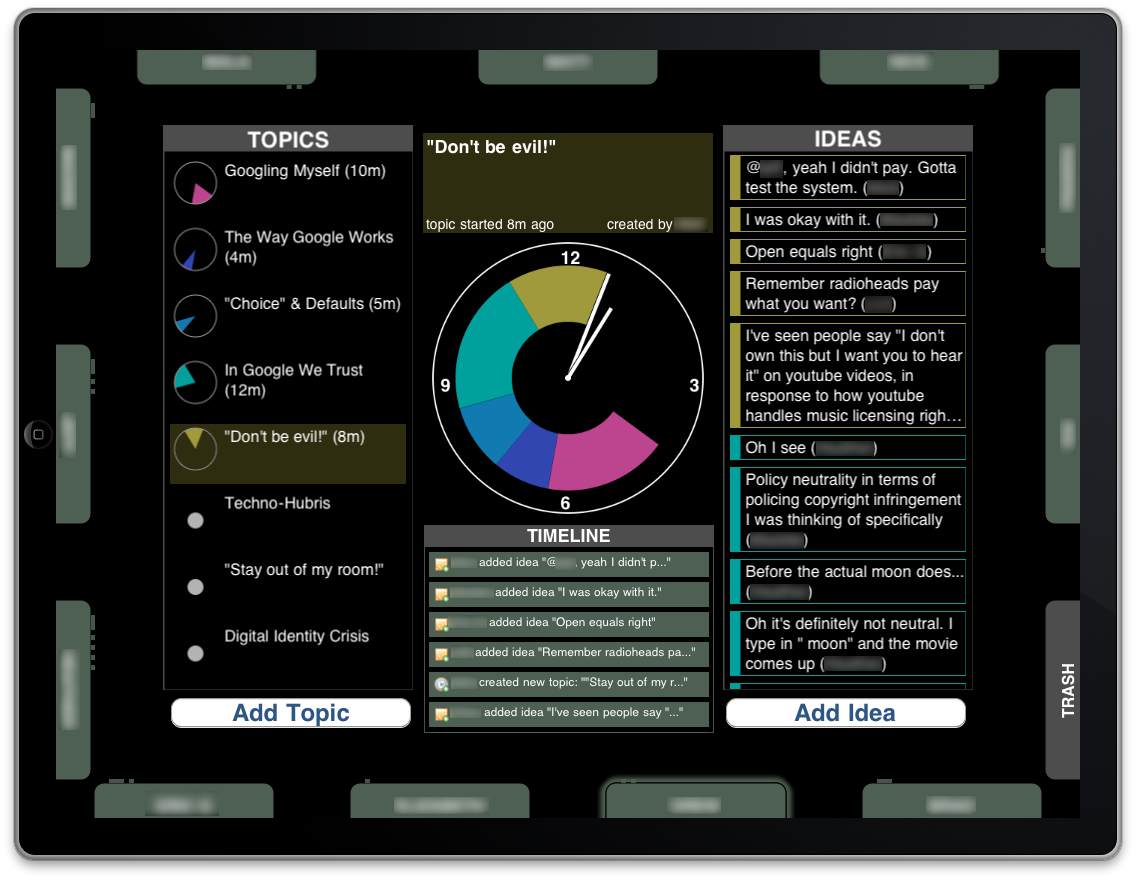
\includegraphics[width=8cm]{tincan_ui.png}
\caption{Benutzerobefläche Tin Can (entnommen von [12])}
\label{tincan_ui}
\end{figure}

Damit sind persönliche Ideen per Definition nichts privates. Sie bieten dem
Benutzer eher eine Möglichkeit, seine Zurückhaltung bei einer Idee auszudrücken.


\subsection{Evaluation}
Harry et al. \cite{HarGorSch2012} führten eine Studie mit zwei Seminaren über 6 Wochen durch. Dabei
bestand eine Gruppe am Morgen aus 8 Studierenden und eine zweite Gruppe am
Nachmittag aus 11 Studierenden. In die Studie flossen die Beobachtungen der
Seminare, Aufzeichnungen der mit Tin Can erfassten Sitzungen sowie
semistrukturierte Interviews ein.

Auf eine Video- oder Sprachaufzeichnung wurde verzichtet, damit dieses
Medium nicht als störender Faktor die Studie verfälscht (man wollte ja eben gerade
nicht die Diskussion stören). Die Beobachtung wurde nicht durch den
Seminarleiter aufgezeichnet sondern durch einen neutralen Beobachter, da der
Gruppenleiter als Teil der Gruppe gesehen werden muß.

Die Aufzeichnung des Beobachters folgten keinem Schema, es wurde alles
aufgezeichnet, von der Position des Tablets bis hin zu dem Verhalten der
Gruppenteilnehmer untereinander.

Die durchgeführte Analyse der aufgezeichneten Sitzungen ergab folgende Kennzahlen (siehe Tabelle \ref{tincan_kennz}):

\begin{table}[htp]
  \begin{tabular}{ l  l }
    Sitzungsdauer \O & 105 Min.\\
    \\
    Ideen  (gesamt) &  839 \\
    Ideen  (veröffentlicht durch Prof.) & 57\% \\
    \\
    Themen (erstellt) & 119 \\
    Themen (diskutiert) & 79 \\
    Themen (direkt veröffentlicht) & 72\% \\
    Themen (später veröffentlicht) & 5\% \\ 
    Themen (unveröffentlicht) & 23\% \\
    \\
    Themen (Sitzung) \O & 6,5 \\
    Themen (Sitzung) $\pm$ & 2,3 \\
    Themendauer \O & 851 Sek. \\
    Themendauer $\pm$ & 673 Sek. \\
  \end{tabular}
  \caption{Kennzahlen der Tin Can Studie}
  \label{tincan_kennz}
\end{table}

Auffallend waren hier zwei Kennzahlen: Die hohe Abweichung der Themendauer von
673  sec wurde von den Autoren durch die vielen kurzen Themen erklärt, welche zu
der Verzerrung der Verteilung führten.

Die zweite Anomalie war die ungleichmäßige Verteilung von Themen gesehen über
die Zeit. Die Studie kommt zu dem Ergebnis, dass dies eine vorhersehbare 'bursty
structure' Verteilung im klassischen Sinne des Begriffs von Kleinberg
\cite{Klei2003} ist.

Die Interviews zeigten, dass Tin Can die Möglichkeit einer Nebenbühne bietet,
nicht aber den Zwang diese zu benutzen. Das Hauptproblem für die
Studienteilnehmer war, die Balance zwischen der Haupt- und Nebenbühne zu finden,
ohne sofort unaufmerksam zu wirken.

Ebenso wurde als positiv empfunden, dass man die Diskussion auf der Second-Stage
nicht unbedingt verfolgen musste, da man ja nach Ende der Diskussion eine
Zusammenfassung gemailt bekommt.

Der Dozent nutzte Tin Can oft um das Feedback an seinem Vortrag live zu messen
und die Moderation gezielter zu führen, indem er z.B. die privaten Ideen
aufgreift und die Autoren diese Themas motiviert, an der Diskussion teilzunehmen.

Negativ bewerteten die Teilnehmer die Texteingabe auf dem Tablet, welche oft
als nicht schnell genug empfunden wurde um mit der Diskussion mithalten zu können.

Die Studie zeigt, dass das duale Stagekonzept schüch\-ter\-nen, eher als 'Denker'
beschriebenen, Charakteren die Chance gibt, ihren Beitrag auf der Side-Stage zu
posten und so an der Diskussion teilzunehmen. Dabei ist nicht immer mangelndes
Selbstvertrauen in den Interviews genannt worden, sondern oft auch der Wunsch
nicht störend in den Hauptvortrag eingreifen zu wollen.

Die Möglichkeit Ideen zu teilen, eigene Ideenlisten zu füh\-ren und Ideen
anderer aufzugreifen, wurde besonders von den Dozenten geschätzt, um die Beteiligung durch
direkte Ansprache der Teilnehmer zu erhöhen. Teilnehmer wurden durch die direkte
Integration sowie durch Bewertung ihrer Ideen von anderen Teilnehmern
motiviert, sich mehr zu beteiligen.

Die Studie belegt, dass beide Ziele des Projekts Tin Can erfolgreich umgesetzt
werden konnten, da sowohl Ideen- und Themenvielfalt als auch die
Diskussionsteilnahme nachweislich verbessert werden konnten.

Allerdings kommt die Studie auch zu dem Schluss, dass es eine kritische Masse im
Sinne der Gruppengröße gibt. In zu kleinen Gruppen kann Tin Can nicht richtig
funktionieren, da die Nebenbühne einen Teil der gesamten Aufmerksamkeit fordert. 
Bei größeren Gruppen gibt es immer mal wieder Zeit, sich von der Hauptbühne auf
die Nebenbühne zu konzentrieren da es mehr Wechselzeiten gibt (z.B. zwischen
verschiedenen Sprechern, etc.)





